\section{Neural Networks}\label{sec:neural-networks}
Without further ado, we will discuss what neural networks are and how they are composed.
We describe what a layer is and what types there are.
For what do we need optimizers and activation functions and what types are there.
Neural Networks are useful in a multitude of fields like classification, regression, transcription, or machine translation. \cite{goodfellow_deep_2016}
Neuronal networks are composed of layers, which are composed of neurons.
The neuron is the computational component in a deep neural network.\\
A neuron transforms a vector of inputs $\mathbf{x}$ to the output $y$, $\mathbb{R}^n \to \mathbb{R}$
by using a vector of weights $\mathbf{w}$, a bias $b$ and an activation function $f$ \ref{eq: NeuralFunction}.
\begin{equation}
    y = f\left( \sum^n_{i=1} w_i\cdot x_i + b\right)
    \label{eq: NeuralFunction}
\end{equation}
For Example, in the machine learning software library TensorFlow, which is based on Keras, uses by default Glorot uniform initializer\cite{noauthor_tfkeraslayersdense_2023,glorot_understanding_2010},
also called Xavier uniform initializer for the weights and initializes the bias with zeros.\\
Another important component, are the activation functions, one of the most common ones is the sigmoid function, which is today mostly used in output layers.
The rectified linear unit, short ReLU \ref{eq: relu} which was first used 1975 by Fukushima\cite{fukushima_cognitron_1975} and shown in 2011 by Glorot et al. \cite{glorot_deep_2011}
that it enables a better training for a neural network compared to the till then common sigmoid function.
\begin{equation}
    f(x) =
    \begin{cases}
        x& x > 0\\
        0& x <= 0
    \end{cases}
    \label{eq: relu}
\end{equation}
Another even more promising activation function is the Gaussian Error Linear Unit, short GELU \ref{eq: relu} which was proposed by Hendrycks and Gimpel in 2016\cite{hendrycks_gaussian_2016} is used by natural language processing models like BERT\cite{devlin_bert_2019}.
It does not just set all negative values to zero like ReLU but weights them.
The differences can be seen in the figure. \ref{fig: activation function}
\begin{equation}
    f(x) = 0.5x\left ( 1+\tanh\left [ \sqrt{\frac{2}{\pi}}\left ( x+0.044715x^3 \right ) \right ] \right )
    \label{eq: gelu}
\end{equation}
\begin{figure}
    \centering
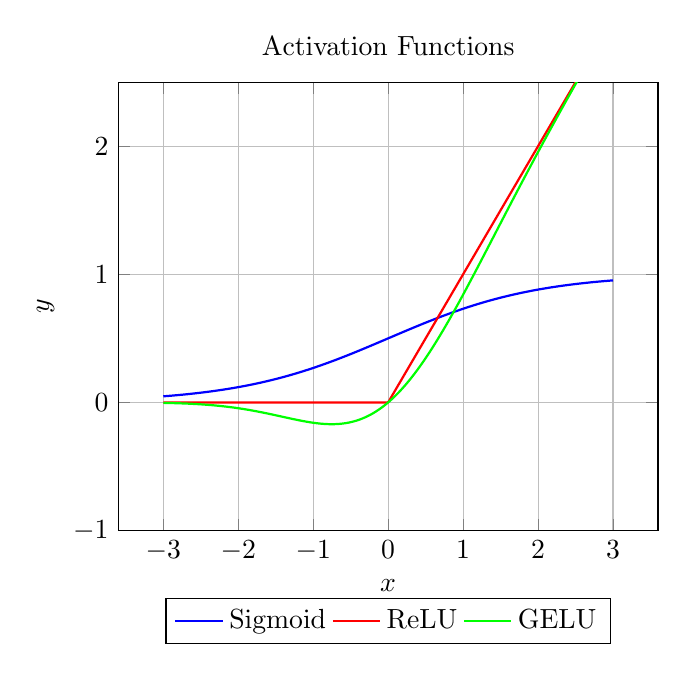
\begin{tikzpicture}
    \begin{axis}[
        title={Activation Functions},
        xlabel={$x$},
        ylabel={$y$},
        domain=-3:3, % Adjust the domain for a narrower x-axis range
        ymin=-1, % Set y-minimum
        ymax=2.5, % Set y-maximum
        samples=400, % Increase the number of samples for a smoother curve
        grid=both,
        legend style={at={(0.5,-0.15)}, anchor=north,legend columns=3},
      ]
      \addplot[blue, thick] {1/(1 + exp(-x))};
      \addplot[red, thick] {max(0, x)};
      \addplot[green, thick] {0.5*x*(1 + tanh(sqrt(2/pi)*(x + 0.044715*x^3)))};
      \legend{Sigmoid, ReLU, GELU}
    \end{axis}
  \end{tikzpicture}
  \caption{Activation Functions}
  \label{fig: activation function}
\end{figure}
The neurons are then combined into layers, in a Deep Neural Network (DNN) we have three types of Layers:
Input layers, output layers and the hidden layers.
In general are there is only one input and one output layer \ref{fig: neural network}, but there is a plurality of hidden layers.
The input layer, is pretty straightforward, it processes the input for the hidden layers, for example, it converts a 2-dimensional picture to a 1-dimensonal array,
which can then be processed by the subsequent layers.
The hidden layer does most of the heavy lifting, it performs most of the computational work of a DNN, it works based on the formula from above.
The output layer, takes the output of the last hidden layer, transforms it so that we get a meaningful output.
For a regression or binary classification, we have mostly just one neuron, but for a multi-class classification the number of neurons corresponds with the number of classes that shall be classified.
The output layer also works after the same principle of the formula above, but not a “normal” activation function is used.
Either a no activation function is used or a linear activation function is used for a regression or the softmax \ref{eq: softmax} function for a classification model.
\begin{equation}
    f(x_i) = \frac{e^{x_i}}{\sum^n_{j=1}e^{x_j}}
    \label{eq: softmax}
\end{equation}
\begin{figure}
  \centering
  % Input layer neurons'number
  \newcommand{\inputnum}{5}

  % Hidden layer neurons'number
  \newcommand{\hiddennuma}{6}
  \newcommand{\hiddennumb}{8}
  \newcommand{\hiddennumc}{5}

  % Output layer neurons'number
  \newcommand{\outputnum}{4}

  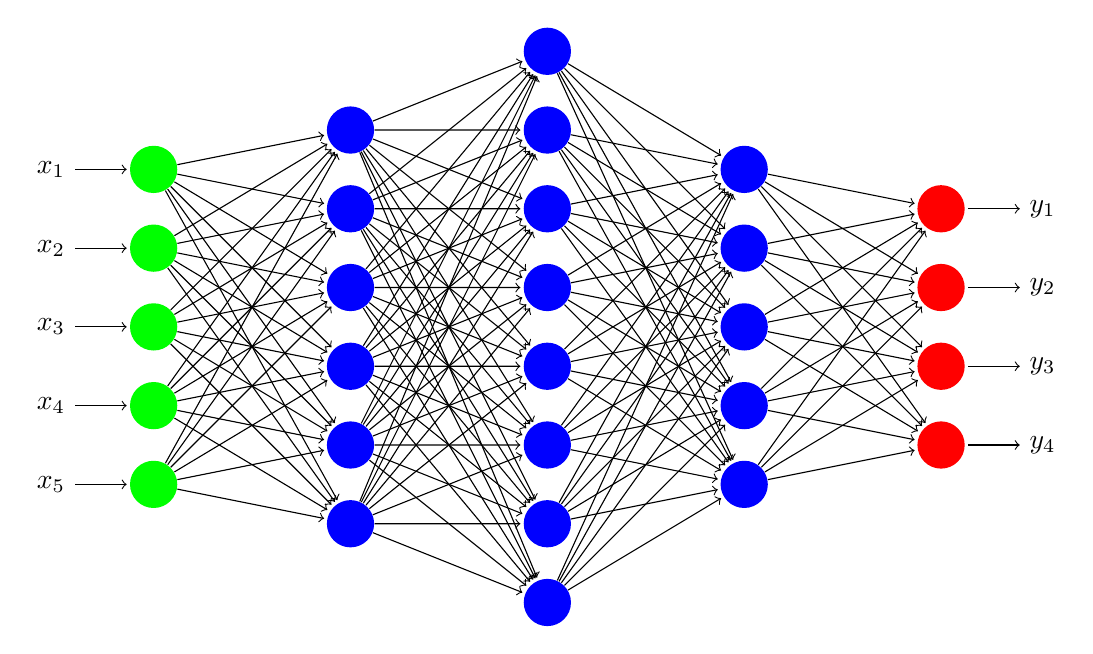
\begin{tikzpicture}

    % Input Layer
    \foreach \i in {1,...,\inputnum}
    {
	  \node[circle,
		minimum size = 6mm,
		fill=green] (Input-\i) at (0,-\i) {};
    }

    % Hidden Layer
    \foreach \i in {1,...,\hiddennuma}
    {
      \node[circle,
		minimum size = 6mm,
		fill=blue,
		yshift=(\hiddennuma-\inputnum)*5 mm
	  ] (HiddenA-\i) at (2.5,-\i) {};
    }

    \foreach \i in {1,...,\hiddennumb}
    {
	  \node[circle,
		minimum size = 6mm,
		fill=blue,
		yshift=(\hiddennumb-\inputnum)*5 mm
	  ] (HiddenB-\i) at (5,-\i) {};
    }

    \foreach \i in {1,...,\hiddennumc}
    {
	  \node[circle,
		minimum size = 6mm,
		fill=blue,
		yshift=(\hiddennumc-\inputnum)*5 mm
	  ] (HiddenC-\i) at (7.5,-\i) {};
    }

    % Output Layer
    \foreach \i in {1,...,\outputnum}
    {
	  \node[circle,
		minimum size = 6mm,
		fill=red,
		yshift=(\outputnum-\inputnum)*5 mm
	  ] (Output-\i) at (10,-\i) {};
    }

    % Connect neurons In-Hidden
    \foreach \i in {1,...,\inputnum}
    {
	  \foreach \j in {1,...,\hiddennuma}
	  {
		\draw[->, shorten >=1pt] (Input-\i) -- (HiddenA-\j);
	  }
    }

    % Connect neurons Hidden
    \foreach \i in {1,...,\hiddennuma}
    {
	  \foreach \j in {1,...,\hiddennumb}
	    {
		  \draw[->, shorten >=1pt] (HiddenA-\i) -- (HiddenB-\j);
	  }
    }

    \foreach \i in {1,...,\hiddennumb}
    {
	  \foreach \j in {1,...,\hiddennumc}
	    {
		  \draw[->, shorten >=1pt] (HiddenB-\i) -- (HiddenC-\j);
	  }
    }

    % Connect neurons Hidden-Out
    \foreach \i in {1,...,\hiddennumc}
    {
	  \foreach \j in {1,...,\outputnum}
	    {
		\draw[->, shorten >=1pt] (HiddenC-\i) -- (Output-\j);
	}
  }

  % Inputs
  \foreach \i in {1,...,\inputnum}
    {
	  \draw[<-, shorten <=1pt] (Input-\i) -- ++(-1,0)
		node[left]{$x_{\i}$};
    }

  % Outputs
  \foreach \i in {1,...,\outputnum}
    {
	  \draw[->, shorten <=1pt] (Output-\i) -- ++(1,0)
		node[right]{$y_{\i}$};
    }

  \end{tikzpicture}
  \caption{Neural Network}
  \label{fig: neural network}
  \fcolorbox{black}{green}{\rule{0pt}{6pt}\rule{6pt}{0pt}}\quad Input Layer \quad
  \fcolorbox{black}{blue}{\rule{0pt}{6pt}\rule{6pt}{0pt}}\quad Hidden Layer \quad
  \fcolorbox{black}{red}{\rule{0pt}{6pt}\rule{6pt}{0pt}}\quad Output Layer
\end{figure}
But, how are deep neural networks trained? \cite{lecun_deep_2015}
The first step is forward propagation, the training data is fed in to the network and flows through the layers, where each neuron performs it operation. \ref{eq: NeuralFunction}
Afterward the backpropagation or backpropagation of error is performed. \cite{rumelhart_learning_1986}
Then the output is compared to the desired outcome of the training data, hence, if the predicted outcome of the network matches the actual outcome.
If it doesn't match, it calculates how far off the prediction is.
The process of backpropagation is initiated, which uses an algorithm like Stochastic Gradient Descent (SGD) or one of its modern successors like Adam.
SGD updates the model parameters by using the gradient of the loss function concerning the parameter.
This isn't done for the whole dataset but just some data points.
The learning rate describes how far a parameter is changed in the direction of a derivation for one iteration, in SGD this Learning Rate is constant and manually set.

Adaptive Moment Estimation (Adam)\cite{kingma_adam_2017} is one of the successors of SGD. Adam, uses a variable learning rate which is adapted for each parameter, which uses the estimation of the first moment, the mean, and the second moment, the variance to change the learning rate.

Then this process is repeated until we are gone through the entire training set, which is called an epoch.

\subsection{Core Layers in Neural Networks}\label{subsec:core-layers-in-neural-networks}

\subsubsection{Dense Layers}
Dense Layers are the backbone of neural networks.
They do most of the computational work of a neural network.
It's characterized by its fully connected architecture, like seen in the figure \ref{fig: neural network}, meaning every node of the layer is connected to every node of the predecessor layer and every node of the successor layer.
Dense layers are pivotal in learning intricate patterns from data, their versatility allows them to be stacked where each layer captures different levels of data abstraction.
They work internally, like in the function above \ref{eq: NeuralFunction}.

\subsubsection{Convolutional Layer}
Convolutional layers, are used in image processing\cite{lecun_backpropagation_1989,szegedy_going_2014,krizhevsky_imagenet_2012}, unlike dense layers that try to analyse an image as a whole, but uses the concept of convolution to get a set of smaller pictures which depict isolated features of a picture.
A convolution describes how a function f is modified by a function g, for example in the discrete case: \ref{eq: convolution}.
\begin{equation}
(f \ast g)[n]
    = \sum_{m=-\infty}^{\infty}f[m]\cdot g[n - m]
    \label{eq: convolution}]
\end{equation}
But how does this correspond to neural networks and image processing, foremost, we have not 1Dimensional data, but 2Dimensional pictures. \ref{eq: 2Dconvolution} \ref{fig: convolution matrix}
\begin{equation}
(f \ast g)[x,y]
    = \sum^{\infty}_{m=-\infty} \sum^{\infty}_{n=-\infty} f[m,n]\cdot g[x-m,y-n]
    \label{eq: 2Dconvolution}
\end{equation}
\begin{figure}
\centering
\begin{tikzpicture}[
    2d-arr/.style={matrix of nodes, row sep=-\pgflinewidth, column sep=-\pgflinewidth, nodes={draw}}
  ]

  \matrix (mtr) [2d-arr] {
  0 & 1 & 1 & |[fill=red!30]| 1 & |[fill=red!30]| 0 & |[fill=red!30]| 0 & 0\\
  0 & 0 & 1 & |[fill=red!30]| 1 & |[fill=red!30]| 1 & |[fill=red!30]| 0 & 0\\
  0 & 0 & 0 & |[fill=red!30]| 1 & |[fill=red!30]| 1 & |[fill=red!30]| 1 & 0\\
  0 & 0 & 0 & 1 & 1 & 0 & 0\\
  0 & 0 & 1 & 1 & 0 & 0 & 0\\
  0 & 1 & 1 & 0 & 0 & 0 & 0\\
  1 & 1 & 0 & 0 & 0 & 0 & 0\\
  };

  \node[below=of mtr-5-4] {$\mathbf F$};

  \node[right=0.2em of mtr] (str) {$*$};

  \matrix (K) [2d-arr, right=0.2em of str, nodes={draw, fill=green!30}] {
    1 & 0 & 1 \\
    0 & 1 & 0 \\
    1 & 0 & 1 \\
  };
  \node[below=of K-3-2] {$\mathbf G$};

  \node[right=0.2em of K] (eq) {$=$};

  \matrix (ret) [2d-arr, right=0.2em of eq] {
  1 & 4 & 3 & |[fill=blue!80!black!30]| 4 & 1\\
  1 & 2 & 4 & 3 & 3\\
  1 & 2 & 3 & 4 & 1\\
  1 & 3 & 3 & 1 & 1\\
  3 & 3 & 1 & 1 & 0\\
  };
  \node[below=of ret-4-3] {$\mathbf{F * G}$};

  \draw[dashed, red] (mtr-1-6.north east) -- (K-1-1.north west);
  \draw[dashed, red] (mtr-3-6.south east) -- (K-3-1.south west);

  \draw[dashed, blue!80!black] (K-1-3.north east) -- (ret-1-4.north west);
  \draw[dashed, blue!80!black] (K-3-3.south east) -- (ret-1-4.south west);

  \foreach \i in {1,2,3} {
      \foreach \j in {4,5,6} {
          \node[font=\tiny, scale=0.6, shift={(-1.2ex,-2ex)}] at (mtr-\i-\j) {$\times \pgfmathparse{int(mod(\i+\j,2))}\pgfmathresult$};
        }
    }

\end{tikzpicture}
\caption{Example Convolution}
\label{fig: convolution matrix}
    Figure based on a post by Riebesell. \cite{riebesell_convolution_2022}
\end{figure}
For this, the singular weights are replaced by matrices of weights, so-called kernels or filters.
The output of the convolutional layer, are so-called feature maps, each of these contains the result of applying one filter to the input data.
These capture different aspects, like edges or textures.
There are two other variables in a convolutional layer, apart from the number of the number and size of filters and the activation function.
They are the stride and the padding, the stride describes how many steps the filter moves between successive convolutions.
The larger stride, the smaller the resulting filter map, and vice versa.
Of course, a larger stride results in less detail in a map.
Padding is an optional parameter which aids in maintaining information on the edge of an input and helps to keep the scale of a picture.

\subsubsection{Pooling Layer}
Pooling is an often used concept in Convolutional Neural Networks to reduce the size of the individual feature map produced by the convolutional layer, while conserving important details of the feature map.
Especially to produce an output which has a similar size as the input, a pooling layer can be avoided \cite{jain_supervised_2007}.
There are multiple types of pooling operations, but the most used ones are Max-Pooling \ref{fig: Max Pooling} and Average-Pooling \ref{fig: Average Pooling}.
Which operation is best depends on the type of data to be analysed and its pooling cardinality, which describes the number of extracted features.
There can be said, for smaller cardinalities a Max-Pooling should be used, for larger ones Average-Pooling \cite{boureau_theoretical_2010}.
In the complex layer terminology \cite{goodfellow_deep_2016} there are, the convolution stage, the detector stage (Which is just the usage of a nonlinear activation function) and the pool stage, these stages are sublayers of the large convolutional layer.
In the simple layer terminology, those three are all individual layers.
\begin{figure}[h]
\centering
\begin{tikzpicture}[
    2d-arr/.style={matrix of nodes, row sep=-\pgflinewidth, column sep=-\pgflinewidth, nodes={draw}}
  ]

  \matrix (mtr) [2d-arr] {
  |[fill=red!30]| 3 & |[fill=red!30]| 4 & |[fill=blue!30]| 6 & |[fill=blue!30]| 7\\
  |[fill=red!30]| 4 & |[fill=red!30]| 1 & |[fill=blue!30]| 2 & |[fill=blue!30]| 9\\
  |[fill=green!30]| 6 & |[fill=green!30]| 6 & |[fill=yellow!30]| 2 & |[fill=yellow!30]| 3\\
  |[fill=green!30]| 7 & |[fill=green!30]| 1 & |[fill=yellow!30]| 6 & |[fill=yellow!30]| 5\\
  };

  \node[right=0.2em of mtr] (str) {$\Longrightarrow$};

  \matrix (K) [2d-arr, right=0.2em of str] {
    |[fill=red!30]| 4 & |[fill=blue!30]| 9 \\
    |[fill=green!30]| 7 & |[fill=yellow!30]| 6 \\
  };

\end{tikzpicture}
\begin{tikzpicture}[
    2d-arr/.style={matrix of nodes, row sep=-\pgflinewidth, column sep=-\pgflinewidth, nodes={draw}}
  ]

  \matrix (mtr) [2d-arr] {
  |[fill=red!30]| 3 & |[fill=red!30]| 4 & |[fill=blue!30]| 6 & |[fill=blue!30]| 7\\
  |[fill=red!30]| 4 & |[fill=red!30]| 1 & |[fill=blue!30]| 2 & |[fill=blue!30]| 9\\
  |[fill=green!30]| 6 & |[fill=green!30]| 6 & |[fill=yellow!30]| 2 & |[fill=yellow!30]| 3\\
  |[fill=green!30]| 7 & |[fill=green!30]| 1 & |[fill=yellow!30]| 6 & |[fill=yellow!30]| 5\\
  };

  \node[right=0.2em of mtr] (str) {$\Longrightarrow$};

  \matrix (K) [2d-arr, right=0.2em of str] {
    |[fill=gray!30]| 9\\
  };
\end{tikzpicture}
\caption{Max Pooling}
\label{fig: Max Pooling}
Left: Max Pooling, Filter: (2,2) Stride: 2 Right: Max Global Pooling
\end{figure}
\begin{figure}[h]
\centering
\begin{tikzpicture}[
    2d-arr/.style={matrix of nodes, row sep=-\pgflinewidth, column sep=-\pgflinewidth, nodes={draw}}
  ]

  \matrix (mtr) [2d-arr] {
  |[fill=red!30]| 3 & |[fill=red!30]| 4 & |[fill=blue!30]| 6 & |[fill=blue!30]| 7\\
  |[fill=red!30]| 4 & |[fill=red!30]| 1 & |[fill=blue!30]| 2 & |[fill=blue!30]| 9\\
  |[fill=green!30]| 6 & |[fill=green!30]| 6 & |[fill=yellow!30]| 2 & |[fill=yellow!30]| 3\\
  |[fill=green!30]| 7 & |[fill=green!30]| 1 & |[fill=yellow!30]| 6 & |[fill=yellow!30]| 5\\
  };

  \node[right=0.2em of mtr] (str) {$\Longrightarrow$};

  \matrix (K) [2d-arr, right=0.2em of str] {
    |[fill=red!30]| 3 & |[fill=blue!30]| 6 \\
    |[fill=green!30]| 5 & |[fill=yellow!30]| 4 \\
  };

\end{tikzpicture}
\begin{tikzpicture}[
    2d-arr/.style={matrix of nodes, row sep=-\pgflinewidth, column sep=-\pgflinewidth, nodes={draw}}
  ]

  \matrix (mtr) [2d-arr] {
  |[fill=red!30]| 3 & |[fill=red!30]| 4 & |[fill=blue!30]| 6 & |[fill=blue!30]| 7\\
  |[fill=red!30]| 4 & |[fill=red!30]| 1 & |[fill=blue!30]| 2 & |[fill=blue!30]| 9\\
  |[fill=green!30]| 6 & |[fill=green!30]| 6 & |[fill=yellow!30]| 2 & |[fill=yellow!30]| 3\\
  |[fill=green!30]| 7 & |[fill=green!30]| 1 & |[fill=yellow!30]| 6 & |[fill=yellow!30]| 5\\
  };

  \node[right=0.2em of mtr] (str) {$\Longrightarrow$};

  \matrix (K) [2d-arr, right=0.2em of str] {
    |[fill=gray!30]| 4.5\\
  };

\end{tikzpicture}
\caption{Average Pooling}
\label{fig: Average Pooling}
Left: Average Pooling, Filter: (2,2) Stride: 2 Right: Average Global Pooling
\end{figure}

Now, with the usage of the convolutional layer and the pooling layer, we can preprocess data to get better results with the dense layers, which we still need to classify our data.


\section{Neural Network Testing}\label{sec:neural-network-testing}
The testing methods can be categorized into two distinct categories, which are akin to testing in conventional software.
They are coverage criteria and test case generation.
In the subsequent section, we shall examine various methodologies employed for testing singular deep neural networks.\cite{huang_survey_2020}

But first, how do we define an erroneous behaviour of a neural network? \ref{eq: erroneous behaviour}

Where $f: \mathbb{R}^{s_1} \to \mathbb{R}^{s_K}$ is a trained neural network, $\mathcal{H}: \mathbb{R}^{s_1} \to \mathbb{R}^{s_K}$ and a legitimate input $x \in \mathbb{R}^{s_1}$, then we define the erroneous behaviour as:
\begin{equation}
    \arg \max_{j} f_j (x) \neq \arg \max_{j} \mathcal{H}_j (x)
    \label{eq: erroneous behaviour}
\end{equation}

\subsection{Coverage Criteria}\label{subsec:coverage-criteria}
We need the coverage criteria to get a quantitative basis for deciding how thoroughly our neural network is tested and to ensure that in our network key aspects aren't overlooked.
Of course, the criteria used in neural network testing differ from those in software testing.

\subsubsection{Neuron Coverage}
Neuron coverage is the most basic coverage criteria, it is the ratio of the number of neurons activated by the test cases to the total number of neurons in the network.
A neuron is activated if the output of the neuron is greater than zero.
The neuron coverage is equivalent to the statement coverage in software testing, it helps to measure the thoroughness of the test cases.

\subsubsection{Safety Coverage}
The Safety Coverage is derived, by discretizing the input space into a set of hyper-rectangles, each of these hyper-rectangles exhibit the same pattern of activations of neurons, because it has a similar feature set.
A hyper-rectangle is considered safely covered if a test case is classified correctly for all points in the hyper-rectangle.
\subsubsection{Modified Condition/Decision Coverage}
Modified Condition/Decision Coverage (MC/DC) is a method in software testing, which requires that each condition in a decision is tested independently and that each condition is shown to affect the decision outcome independently.
This is done by varying the input of the condition while holding the other conditions constant.
The method is particularly useful in identifying cases where multiple conditions contribute to a decision's outcome.
By using a sign change and a value change to change, it's tried to exploit the relationship between those and use these as a coverage criterion.
\subsubsection{Quantitative Projection}
Quantitative Projection Coverage, is based on the assumption that the input differs on some kind of operation condition.
For example, for self-driving cars: weather, landscape or impeding items.

\subsection{Test Case Generation}
But how do we now generate our test case, to get some useful information?
We have, of course, multiple methods to generate our test cases:

\subsubsection{Input Mutation}
Input Mutation, is a method where we take one of the inputs and transform it, by some predefined rules, to generate our test cases.
For example, in combination with safety coverage, we try to mutate the input in that way so that we cover every hyper-rectangle.
\subsubsection{Fuzzing}
Fuzzing, is a method where we generate random inputs, which are modified from the input set, those are then fed into the network.
There by, we try to cover as much of the input space as possible.
This can help us because a neural network, is designed for high-dimensional data, aim is to find cases where these small changes to the input cause the DNN to fail or behave unexpectedly.

\subsubsection{Symbolic Execution}
Despite the efficacy of input mutation and fuzzing in generating a substantial quantity of random data, it is uncertain whether certain test objectives will be fulfilled.
With Symbolic Execution, we try to find out which input causes a part of a program to execute.
One approach in Symbolic Execution is concolic testing, which is a hybrid testing technique which is adapted for neural networks with DeepConcolic.
Concolic testing combines the concrete execution of a program, with random input generation, hence symbolic data.
There by, the findings of the first step are used to generate the second set of inputs.

\section{Spectrum Analysis}\label{sec:spectrum-analysis}
Another important detail that requires introduction, Spectrum-Based Fault Localization (SBFL)\cite{wong_handbook_2023}, it is a technique to identify the source of faults in software.
The term spectrum, describes in this context the execution profile of the program, which is collected during the execution of a test suite.
During the execution, the coverage of each statement by a test case is recorded and if this test case is a success or a failure.
\begin{table}
\centering
\begin{tabular}{|c|c|c|c|}
\hline
\multicolumn{2}{|c|}{} & \multicolumn{2}{c|}{\textbf{Is the statement covered?}}\\
\cline{3-4}
\multicolumn{2}{|c|}{} & \textbf{Yes (1)} & \textbf{No (0)}  \\ \hline
\multirow{2}{*}{\textbf{Execution result}} & \textbf{Failed (0)} &$a_{ef}$ & $a_{nf}$\\
 & \textbf{Successful (1)} & $a_{es}$ & $a_{ns}$\\ \hline
\end{tabular}
\caption{Symbols used in coefficients}
\label{tab: Sus symbols}
\end{table}
First, only failed test cases were recorded for SBFL, but later also successful test cases were recorded, which provide us with the information of the contrast between failure and success, which aids us to identify truly faulty statements.
For example, in the first case, code that is often executed or every time, would be marked faulty simply for being in a programme.
In the second case, the code wouldn't be marked faulty because it is also executed frequently in successful test cases.
The term “code coverage” is frequently referred to as “executable statement hit spectrum” (ESHS), which denotes the extent to which certain components of the program under testing have been covered during execution.
Some popular ESHS-based are based on a similarity coefficient, for example Tarantula\cite{jones_empirical_2005} \ref{eq: tarantula} , Ochiai\cite{ochiai_zoogeographical_1957} \ref{eq: ochiai} or Dstar\cite{wong_dstar_2014} \ref{eq: dstar} (Often also called $D^*$, where $*$ denotes the used exponent).
\begin{equation}
    \frac{\frac{a_{ef}}{a_{ef} + a_{nf}}}{\frac{a_{ef}}{a_{ef} + a_{nf}}+\frac{a_{es}}{a_{es} + a_{ns}}}
    \label{eq: tarantula}
\end{equation}
\begin{equation}
    \frac{a_{ef}}{\sqrt{(a_{ef}+a_{nf})\cdot(a_{ef}+a_{es})}}
    \label{eq: ochiai}
\end{equation}
\begin{equation}
    \frac{{a_{ef}}^*}{a_{es}+a_{nf}}
    \label{eq: dstar}
\end{equation}
By the work of Lee et al. \cite{hua_jie_lee_study_2009} \ref{eq: simple_tarantula} the formula for Tarantula could even be more simplified.
Yoo et al. \cite{yoo_human_2017}said that using genetic programming to create ranking metrics can consistently exceed many human-designed ranking metrics, like the once discussed above.
\begin{equation}
    \frac{a_{ef}}{a_{ef}+a_{es}}
    \label{eq: simple_tarantula}
\end{equation}
In the following, you can see an Example \cite{parsa_software_2023} to see what spectrum analysis is, and what a pitfall of this method is.
The code \ref{lst:code_snippet sfl} depicts some simple calculation program, which takes the two integers a and b as input and an integer c for the branching of the calculation.
At line 11, the Max value is wrongly set, this is the fault that needs to be found.
In the table \ref{tab: sfl}, you can see the suspiciousness values calculated with ochiai and tarantula.

But because line 8, is always executed with line 11 and is overall less executed than line 11, it is the more suspicious statement.
Hence, we can see that spectrum analysis isn't the silver bullet, for eradicating faults in programs.
\begin{lstlisting}[caption={Example code snippet}, label={lst:code_snippet sfl}]
int getImpact()
{
    scanf("%d %d %d", &a, &b, &c);
    Impact = 0;
    Division = 1;
    Sum = a + b;
    if ((a > 0) && (b > 0))
        Division = a / b;
    Max = b;
    if (a > b)
        Max = b; // Correct: Max = a;
    if (c == 1)
        Impact = Sum;
    if (c == 2)
        Impact = Division;
    if (c == 3)
        Impact = Max;
    return Impact;
}
\end{lstlisting}
\begin{table}[!h]
\centering
\begin{tabular}{|c|c|c|c|c|}
\hline
Line & $a_{es}$ & $a_{ef}$ & Tarantula & Ochiai \\
\hline
6 & 6 & 6 & 0.5 & 0.71 \\
7 & 6 & 6 & 0.5 & 0.71 \\
8 & 2 & 6 & 0.75 & 0.87 \\
9 & 6 & 6 & 0.5 & 0.71 \\
10 & 6 & 6 & 0.5 & 0.71 \\
11 & 3 & 6 & 0.67 & 0.81 \\
12 & 6 & 6 & 0.5 & 0.71 \\
13 & 1 & 0 & 0.0 & 0.0 \\
14 & 6 & 6 & 0.5 & 0.71 \\
15 & 2 & 0 & 0.0 & 0.0 \\
16 & 6 & 6 & 0.5 & 0.71 \\
17 & 3 & 6 & 0.67 & 0.81 \\
18 & 6 & 6 & 0.5 & 0.71\\
\hline
\end{tabular}
\caption{Fault values, for code snippet}
\label{tab: sfl}
\end{table}

There are even more similarity coefficients, to an extent which wouldn't be feasible to be covered in this work, an extensive can be referred to by Wong et al. \cite{wong_survey_2016}.

There are some other examples of SBFL, which don't use ESHS, for example Program Invariants Hit Spectrum, which the coverage of program invariants.
Those individuals attempt to identify violations of program properties in failed program executions to locate bugs.
Another one would be the Method Calls Sequence Hit Spectrum, which collects information about the sequence of method calls, during a test-case.

\section{DeepFault}\label{sec:deepfault}
DeepFault\cite{eniser_deepfault_2019} is a white-box testing approach for neural networks, developed by Eniser et al. which is according to the Authors.
\begin{quote}
    ... the first fault localization-based white-box testing approach for DNNs.
\end{quote}
There are two objectives to the approach, the identification of suspicious neurons, which have undesirable behaviour, where the respective neuron is suspected to lead to an undesirable outcome in the whole network.
And the synthesis of new inputs for the neural network, to specially retrain the (most) suspicious values.

\subsection{Identification of suspicious neurons}\label{subsec:identification-of-suspicious-neurons}
In this First Part, DeepFault is establishing a Hit Spectrum($HS$) \ref{eq:hit_spectrum} for all neurons, which take the form of a tuple.
Of course, the input, and output layers are left out because they are considered inherently correct.
\begin{equation}
    HS_n = (attr_n^{as}, attr_n^{af}, attr_n^{ns}, attr_n^{nf}\label{eq:hit_spectrum}
\end{equation}
\begin{itemize}
    \item $attr^{as}_n$ is the number of times the neuron $n$ is activated in successful test cases.
    \item $attr^{af}_n$ is the number of times the neuron $n$ is activated in failed test cases.
    \item $attr^{ns}_n$ is the number of times the neuron $n$ is not activated in successful test cases.
    \item $attr^{nf}_n$ is the number of times the neuron $n$ is not activated in failed test cases.
\end{itemize}
Then the hit spectra are in a suspiciousness measures, in DeepFault Tarantula \ref{eq: tarantula}, Ochiai \ref{eq: ochiai}, $D^3$ \ref{eq: dstar} are used.
These are not used to identify one wrong neuron, but rather a set of wrong neurons.
For that, the suspiciousness values of the neurons are used to sort the neurons in decreasing order of suspiciousness, if multiple neurons happen to get the same value, the neuron in a deeper layer is used.

\subsection{Synthesis of new inputs}\label{subsec:synthesis-of-new-inputs}
Guided by the suspiciousness measures, DeepFault modifies the input, for which the neural network has made the correct decision, in a targeted way.
The synthesis task is supported by a gradient ascent algorithm that aims to determine the degree to which an appropriately classified input should and could be modified to enhance the activation values of suspicious neurons.